L'exercice 20 traite de la construction de suites de disques et de carr{\'e}s.
Il demande de prouver l'existence de suites de carr{\'e}s dans un disque et de
disques dans un carr{\'e}, satisfaisant certaines conditions sur leurs aires
et leurs intersections. L'exercice fait appel {\`a} des notions de
g{\'e}om{\'e}trie et d'analyse.
\begin{exercise}[(Disques et carr{\'e}s)]
Soit $D$ le disque ferm{\'e} de centre 0 et rayon~1 dans~$\mathbb{R}^2$.
Montrer qu'il existe une suite $C_0, C_1, \ldots$ de carr{\'e}s de
$\mathbb{R}^2$ tels que :
\begin{enumerate}
  \item $\forall i \geq 0, C_i \subseteq D$;
  
  \item $\forall i, j \geq 0 : i \neq j \Rightarrow \ring{C}_i \cap \ring{C}_j
  = \varnothing$;
  
  \item $\sum_{i \geq 0} \mathrm{Aire} (C_i) = \pi$.
\end{enumerate}


Soit~$C = [- 1, 1]^2$. Montrer qu'il existe une suite~$D_0, D_1, \ldots$ de
disques de $\mathbb{R}^2$ tels que :
\begin{enumerate}
  \item $\forall i \geq 0, D_i \subseteq C$;
  
  \item $\forall i, j \geq 0 : i \neq j \Rightarrow \ring{D}_i \cap \ring{D}_j
  = \varnothing$;
  
  \item $\sum_{i \geq 0} \mathrm{Aire} (D_i) = 4$.
\end{enumerate}
\end{exercise}

\subsection*{Solution. (ZINE Akram)}
\addcontentsline{toc}{subsection}{Solution. (ZINE Akram)}


\tmtextbf{Lemme 1.} Pour chaque point $(x, y) \in \mathbb{R}^2$ et pour tout
entier $n \geq 1$, il existe au plus deux carr{\'e}s dyadiques de taille $2^{-
n}$ qui contiennent le point $(x, y)$, et ce point ne peut {\^e}tre
int{\'e}rieur {\`a} deux carr{\'e}s en m{\^e}me temps.

\tmtextbf{Preuve du lemme 1.}

Un carr{\'e} dyadique de taille $2^{- n}$ dans $\mathbb{R}^2$ est de la forme
:
\[ C_{k_1, k_2} = \left[ \frac{k_1}{2^n}, \frac{k_1 + 1}{2^n} \right] \times
   \left[ \frac{k_2}{2^n}, \frac{k_2 + 1}{2^n} \right], \]


o{\`u} $k_1, k_2 \in \mathbb{Z}$. Les carr{\'e}s dyadiques forment une grille
qui couvre tout le plan.

Pour chaque point $(x, y) \in \mathbb{R}^2$, nous devons trouver les indices
$k_1, k_2 \in \mathbb{Z}$ tels que le carr{\'e} dyadique $C_{k_1, k_2}$
contient le point. Le crit{\`e}re pour que $(x, y)$ soit dans ce carr{\'e} est
:
\[ \frac{k_1}{2^n} \leq x < \frac{k_1 + 1}{2^n}  \quad \text{et} \quad
   \frac{k_2}{2^n} \leq y < \frac{k_2 + 1}{2^n} . \]


Les indices $k_1$ et $k_2$ qui satisfont les in{\'e}galit{\'e}s ci-dessus sont
donn{\'e}s par :
\[ k_1 = \lfloor 2^n x \rfloor  \quad \text{et} \quad k_2 = \lfloor 2^n y
   \rfloor, \]


o{\`u} $\lfloor \cdot \rfloor$ est la fonction partie enti{\`e}re.

\

1- Pour montrer qu'il existe une suite $\{C_i \}_{i \geq 0}$ de carr{\'e}s
v{\'e}rifiant les conditions donn{\'e}es, nous allons construire cette suite
en nous basant sur des carr{\'e}s dyadiques.

Consid{\'e}rons une suite de disques ferm{\'e}s $D_n$ de centres $0$ et de
rayons $1 - \frac{\sqrt{2}}{2^n}$ pour $n \geq 1$. Ce rayon est choisi pour
que chaque carr{\'e} de cot{\'e} $2^{- n}$ soit contenu {\`a} l'int{\'e}rieur
du disque unit{\'e}.

Chaque disque $D_n$ est contenu dans le disque $D$ de rayon 1, et lorsque $n
\to \infty$, les rayons de ces disques tendent vers 1, couvrant ainsi tout le
disque $D$.

Pour chaque disque $D_n$, nous choisissons un ensemble fini de carr{\'e}s
dyadiques de c{\^o}t{\'e} $2^{- n}$ pour le couvrir, conform{\'e}ment au
lemme. Chaque carr{\'e} dyadique est de la forme :
\[ \left[ \frac{k_1}{2^n}, \frac{k_1 + 1}{2^n} \right] \times \left[
   \frac{k_2}{2^n}, \frac{k_2 + 1}{2^n} \right], \]
o{\`u} $k_1, k_2 \in \mathbb{Z}$. Comme $D_n$ est de taille finie, il peut
{\^e}tre couvert par un nombre fini de ces carr{\'e}s dyadiques de cot{\'e}s
$2^{- n}$.

Nous commen{\c c}ons par couvrir le plus petit disque $C_1$ en utilisant des
carr{\'e}s dyadiques de c{\^o}t{\'e} $2^{- 1} = \frac{1}{2}$.

Ensuite, pour chaque disque suivant $D_{n + 1}$, nous conservons tous les
carr{\'e}s utilis{\'e}s pour couvrir $D_n$ et nous ajoutons de nouveaux
carr{\'e}s dyadiques de c{\^o}t{\'e} $2^{- (n + 1)}$ pour couvrir la partie
non couverte entre $D_n$ et $D_{n + 1}$. (Ceci est possible car deux
carr{\'e}s dyadiques diff{\'e}rents tels que l'un n'est pas inclu dans l'autre
ne peuvent s'intersecter que sur le cot{\'e}).

Les nouveaux carr{\'e}s ajout{\'e}s sont donc de c{\^o}t{\'e} $2^{- (n +
1)}$, plus petits que ceux ajout{\'e}s {\`a} l'{\'e}tape pr{\'e}c{\'e}dente.

L'ensemble des carr{\'e}s $\{C_{n, i} \}$ est index{\'e} par deux indices $n$
et $i$, et peut {\^e}tre vu comme un {\'e}l{\'e}ment de $\mathbb{N}^2$.

{\`A} chaque {\'e}tape $n$, nous avons un ensemble fini de carr{\'e}s
dyadiques qui couvrent le disque $D_n$ {\`a} savoir (($C_{1, 1}, ..., C_{1,
k_1}, ..., C_{n, 1}, ..., C_{n, k_n}$).Puisque $\mathbb{N}^2$ est
d{\'e}nombrable, il existe une bijection entre $\mathbb{N}^2$ et $\mathbb{N}$.

Cela signifie que nous pouvons r{\'e}organiser la suite doublement
index{\'e}e $\{C_{n, i} \}$ en une suite simple $\{C_m \}_{m \in \mathbb{N}}$,
c'est-{\`a}-dire ($C_1, C_2, C_3, \ldots$).

L'union de ces ensembles de carr{\'e}s forme une couverture compl{\`e}te du
disque $D$ lorsque $n \to \infty$.

En effet, ces carr{\'e}s couvrent le disque de rayon $1 -
\frac{\sqrt{2}}{2^n}$, il existe une suite $(k_i)$ telle que pour tout $n \geq
1$
\[ \pi \left( 1 - \frac{\sqrt{2}}{2^n} \right)^2 \leq \sum_{i = 1}^n Aire
   (C_{k_i}) \leq \pi \]


D'o{\`u} le r{\'e}sultat.

\begin{figure}[h]
  \centering
  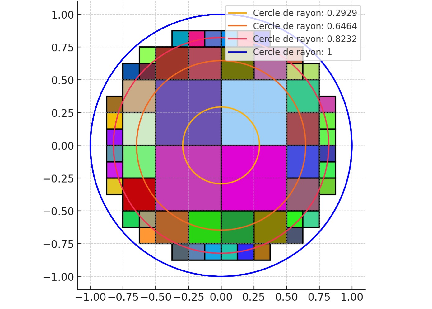
\includegraphics[width=7.249cm,height=5.193cm]{figures/Math_oraux-3.pdf}
  \caption{Carr{\'e}s dyadiques de tailles $1 / 8$, $1 / 4$, et $1 / 2$, ainsi
  que des disques de rayons $1 - \frac{\sqrt{2}}{2^n}$ pour $n = 1, 2, 3$ et
  le disque de rayon 1.}
\end{figure}


2- Soit $C = [- 1, 1]^2$ le carr{\'e} centr{\'e} {\`a} l'origine avec un
c{\^o}t{\'e} de longueur 2. Nous cherchons {\`a} montrer qu'il existe une
suite $\{D_i \}_{i \geq 0}$ de disques disjoints tels que :
\[ \sum_{i \geq 0} \text{Aire} (D_i) = 4. \]


Consid{\'e}rons le carr{\'e} $C$ moins un disque inscrit de rayon 1/2,
centr{\'e} {\`a} l'origine. L'aire de ce disque est donc $\frac{\pi}{4}$.

On commence d'abord par remarquer que tout carr{\'e} dyadique de taille $2^i$
partiellement ext{\'e}rieur {\`a} C ne peut partager une partie avec
l'int{\'e}rieur de C. En effet, empilons dans C $4$ carr{\'e}s dyadiques de
cot{\'e}s $1$.

Ainsi, si un carr{\'e} dyadique partage une partie avec l'int{\'e}rieur C, il
la partage forc{\'e}ment avec l'int{\'e}rieur de l'un de ces $4$ carr{\'e}s,
ce qui est absurde car les carr{\'e}s dyadiques ne peuvent pas se croiser
grace au lemme. \tmtextbf{}

De mani{\`e}re similaire {\`a} la premi{\`e}re partie du probl{\`e}me, la
r{\'e}gion restante dans le carr{\'e} $C$ peut {\^e}tre approxim{\'e}e aussi
pr{\'e}cis{\'e}ment que souhait{\'e} par un nombre fini de carr{\'e}s
dyadiques.

En effet, On va consid{\'e}rer une suite de disques de rayons $\frac{1}{2} +
\frac{\sqrt{2}}{2^{n + 1}}$ avec $n \geq 1$ (Pour qu'ils soient inclus dans le
carr{\'e}). Mais cette fois, on pave la r{\'e}gion entre chaque disque $D_n$
et le carr{\'e} par des carr{\'e}s dyadiques de cot{\'e}s ayant pour longueur
$1 / 2^{n + 1}$, comme pour la premi{\`e}re question, l'observation cl{\'e}
ici est que chaque carr{\'e} qui poss{\`e}de des points dans cette r{\'e}gion
est forc{\'e}ment {\`a} l'ext{\'e}rieur du disque de rayon $1 / 2$. (On pourra
s'en convaincre par in{\'e}galit{\'e} triangulaire).

On pourra ainsi construire une suite de carr{\'e}s dyadiques qui s'empilent
compl{\`e}tement dans la r{\'e}gion entre le carr{\'e} et le disque de rayon
$1 / 2$.

\begin{figure}[h]
  \centering
  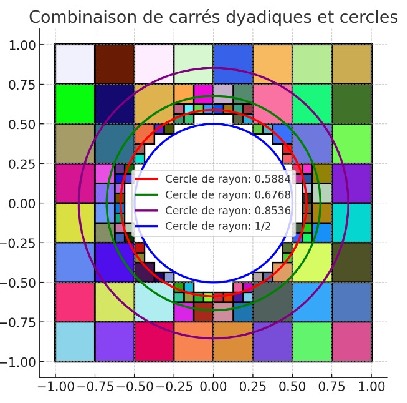
\includegraphics[width=6.831cm,height=6.761cm]{figures/Math_oraux-4.pdf}
  \caption{Carr{\'e}s dyadiques de tailles $1 / 16$, $1 / 8$, et $1 / 4$,
  ainsi que des disques de rayons $1 + \frac{\sqrt{2}}{2^{n + 1}}$ pour $n =
  1, 2, 3$ et le disque de rayon $1 / 2$ dans le carr{\'e} $[-1, 1]^2$.}
\end{figure}


\tmcolor{red}{}On construit la suite de disques par r{\'e}currence avec un
processus diagonal :

Pour $n = 1$, on place dans notre carr{\'e} les carr{\'e}s dyadiques de
cot{\'e} $\frac{1}{2^{n + 1}}$ avec $n = 1$, de fa{\c c}on {\`a} qu'ils ne
soient pas int{\'e}rieur du disque de rayon $\frac{1}{2} +
\frac{\sqrt{2}}{2^{n + 1}}$.

Ces carr{\'e}s sont en nombre fini et correspondent aux carr{\'e}s de niveau 1
pour le carr{\'e} $[- 1, 1]^2$(Voir la figure).

{\`A} l'int{\'e}rieur de ces carr{\'e}s, on place aussi par homoth{\'e}tie
des carr{\'e}s dyadiques de niveau 1 qui contiennent aussi un disque inscrit,
en gardant le m{\^e}me rapport homoth{\'e}tique.

Ces carr{\'e}s contiennent {\`a} leur tour d'autres carr{\'e}s de niveau 1
(c'est le processus diagonal qui permet de construire notre suite disjointe de
disques).

Ensuite, on inscrit des carr{\'e}s dyadiques de niveau 2 dans tous les
carr{\'e}s, et on consid{\`e}re une seconde couche de profondeur,
c'est-{\`a}-dire que dans les carr{\'e}s dyadiques inscrits dans les
carr{\'e}s dyadiques d{\'e}j{\`a} construits, on inscrit deux niveaux de
carr{\'e}s dyadiques suppl{\'e}mentaires, avec leurs disques associ{\'e}s.

On construit ainsi une suite disjointe de disques pour notre carr{\'e},
not{\'e} ($D'_n$).

Pour tout carr{\'e} $C$, on note $D'_n (C) = ((x_n (C), y_n (C), r_n (C)))$ la
suite des disques inscrits dans ce carr{\'e}, en r{\'e}alisant une
homoth{\'e}tie sur la suite construite dans le carr{\'e} $[- 1, 1]^2$.

Introduisons le rapport :
\[ A_C = \frac{\sum_{n = 1}^{\infty} \pi r_n^2 (C)}{\text{aire} (C)} \]


Soit $C$ le carr{\'e} utilis{\'e}. On remarque que $A_C$ ne d{\'e}pend pas du
choix du carr{\'e}, par homoth{\'e}tie. Notons le par $A$. L'aire totale
couverte par les disques est donn{\'e}e par :
\[ 4 A = \frac{\pi}{4} + A \sum_{i = 1}^{\infty} Aire (C_n) = \frac{\pi}{4} +
   \left( 4 - \frac{\pi}{4} \right) A, \]


o{\`u} $\frac{\pi}{4}$ est l'aire du disque inscrit, et $\left( 4 -
\frac{\pi}{4} \right) A$ est l'aire des disques ins{\'e}r{\'e}s dans la suite
des carr{\'e}s dyadiques $C_n$.

On trouve donc que $A = 1$.
\[ \maltese \maltese \maltese \maltese \maltese \maltese \maltese \]
